\chapter{Algorithmen auf Datenstrukturen}

\index{Algorithmus}
\paragraph{Algorithmus} Handlungsvorschrift aus endlich vielen Einzelschritten zur Problemlösung.

% TODO: Link subsections
\begin{itemize}
  \item Korrektheit (Test-based dev.)
  \item Terminierung (\textsc{Touring})
  \item Effizienz (Komplexität)
\end{itemize}

\index{High-level Sprache}
\index{Low-level Sprache}
\paragraph{Formen (High to low)}
Menschl. Sprache, Pseudocode, Mathematische Ausdrücke, Quellcode, Binärcode

\paragraph{Divide \& Conquer}
\index{Divide \& Conquer}

\begin{description}
  \item [Divide] Zerlegen in kleinere Teilprobleme
  \item [Conquer] Lösen der Teilprobleme mit gleicher Methode (rekursiv)
  \item [Merge] Zusammenführen der Teillösungen
\end{description}

\section{Effizienz}
\index{Effizienz}

Raum/Zeit-Tradeoff: schnell + gro\ss vs. klein + langsam.
\index{Raum/Zeit-Tradeoff}

\mzGraphic{
  \begin{tblr}{
    column{2} = {r},
    hline{1-2,4} = {-}{},
      }
    Programmlaufzeit/-allokationen & \emph{Komplexität}    \\
    Einfluss äußerer Faktoren      & Unabh.                  \\
    Konkrete Größe                 & Asymptotische Schätzung
  \end{tblr}
}

\paragraph{Inputgrö\ss e $\mathbf{n}$} Jeweils

\begin{itemize}
  \item Best-case $C_B$
        \index{Best-case Komplexität}
  \item Average-case $C_A$
        \index{Average-case Komplexität}
  \item Worst-case $C_W$
        \index{Worst-case Komplexität}
\end{itemize}

\subsection{Asymptotische Zeit-/Speicherkomplexität}

\index{Gro\ss-O-Notation}
\paragraph{Gro\ss-O-Notation}
Kosten $C_f(n)$ mit $g: \mathbb{N} \rightarrow \mathbb{R} \exists c > 0 \exists n_0 > 0 \forall n \geq n_0$

\begin{description}
  \item [Untere Schranke] $\boldsymbol{\Omega} (f)$ \\
        \index{Untere Schranke Komplexität}
        $C_f(n) \boldsymbol{\geq} c * g(n)$

  \item [Obere Schranke] $\boldsymbol{O}(f)$ \\
        \index{Obere Schranke Komplexität}
        $C_f(n) \boldsymbol{\leq} c * g(n)$

  \item [Exakte Schranke] $\boldsymbol{\Theta} (f)$ \\
        \index{Exakte Schranke Komplexität}
        $C_f(n) \in \Omega (f) \cap O(f)$ \\
        Polynom $k$ten Grades $\in \Theta (n^k)$
\end{description}

(Beweis: $g$ und $c$ finden)

\mzGraphic{
  \begin{tblr}{
    column{4} = {r},
    cell{1}{3} = {c=2}{c},
    cell{2}{4} = {r=6}{},
    cell{6}{3} = {r=2}{},
    cell{8}{4} = {r=3}{},
    vline{3} = {1,7}{},
    vline{3-4} = {2-6,8-10}{},
    hline{1-2,11} = {-}{},
    hline{6,9} = {3}{},
        hline{8} = {3-4}{},
      }
    \emph{Gro\ss-O}\index{Komplexitätsklassen} & \emph{Wachstum} & \emph{Klasse}            &        \\
    $O(1)$          & Konstant          &                            & lösbar \\
    $O(\log n)$     & Logarithmisch     &                            &        \\
    $O(n)$          & Linear            &                            &        \\
    $O(n \log n)$   & Nlogn             &                            &        \\
    $O(n^2)$        & Quadratisch       & Polynomiell $O(n^k)$       &        \\
    $O(n^3)$        & Kubisch           &                            &        \\
    $O(2^n)$        & Exponentiell      & Exponentiell $O(\alpha^n)$ & hart   \\
    $O(n!)$         & Fakultät          &                            &        \\
    $O(n^n)$        &                   &                            &
  \end{tblr}
}

\paragraph{Rechenregeln}

\begin{description}
  \item [Elementare Operationen, Kontrollstr.] $\mathbf{\in O(1)}$
  \item [Schleifen] $\in$ $i$ Wiederholungen $\boldsymbol{*}$ $O(f)$ teuerste Operation
  \item [Abfolge] $O(g)$ nach $O(f)$ $\in O(\boldsymbol{\max} (f;g))$
  \item [Rekursion] $\in$ $k$ Aufrufe $\boldsymbol{*}$ $O(f)$ teuerste Operation
\end{description}

\index{Mastertheorem}
\paragraph{Mastertheorem} $a \geq 1$, $b > 1$, $\Theta > 0$


\begin{gather*}
  T(n) = a * T( \frac{n}{b} ) + \Theta (n^k) \\
  \Rightarrow \begin{cases}
    \Theta ( n^k ) \quad          & a < b^k \\
    \Theta ( n^k * \log n ) \quad & a = b^k \\
    \Theta ( n^{\log_b a} ) \quad & a > b^k
  \end{cases}
\end{gather*}

\paragraph{Floor/Ceiling}

\begin{description}
  \item [Floor] $\floor{x}$ nach unten
        \index{Floor}
  \item [Ceiling] $\ceil{x}$ nach oben
        \index{Ceiling}
\end{description}

\section{Suchverfahren}

\paragraph{Lineare Liste}
\index{Lineare Liste}
endlich, geordnete (nicht sortierte) Folge $n$ Elemente $L := [a_0, \dots, a_n]$ gleichen Typs.

\begin{description}
  \item [Array] Sequenzielle Abfolge im Speicher, statisch, Index $O(1)$, schnelle Suchverfahren
  \item [Verkettet] Zeiger auf nächstes Element, dynamisch, Index $O(n)$,
\end{description}

\index{Sequenzielle Suche}
\paragraph{Sequenziell}
$C_A(n) = \frac{1}{n} * \sum^n i = \frac{n + 1}{2} \in O(n)$\

\begin{algorithm}[H]
  \TitleOfAlgo{Sequential Search}
  \SetKwFunction{Search}{Search}

  \KwIn{Liste $L$, Predikat $x$}
  \KwOut{Index $i$ von $x$}

  \For{$i \leftarrow 0$ \KwTo $L.\text{len} - 1$}{
    \If{$x = L[i]$}{
      \Return{$i$}
    }
  }

  \Return{$-1$}
\end{algorithm}

% TODO: Maximale Teilsumme

\paragraph{Auswahlproblem}
\index{Auswahlproblem}
Finde $i$-kleinstes Element in unsortierter Liste $\in \Theta (n)$

\SetKwFunction{Push}{Push}

\begin{algorithm}[H]
  \TitleOfAlgo{$i$-Smallest Element}
  \SetKwFunction{iSmallestElement}{$i$-Smallest Element}

  \KwIn{Unsortierte Liste $L$, Level $i$}
  \KwOut{Kleinstes Element $x$}

  $p \leftarrow L[L.\text{len} - 1]$

  % $L_{<} \leftarrow []$

  % $L_{>} \leftarrow []$

  \For{$k = 0$ \KwTo $L.\text{len} - 1$}{
    \uIf{$L[k] < p$}{
      \Push ($L_{<}$, $L[k]$)
    }

    \If{$L[k] > p$}{
      \Push ($L_{>}$, $L[k]$)
    }
  }

  \uIf{$L_{<}.\text{len} = i - 1$}{
    \Return {$p$}
  }

  \uIf{$L_{<}.\text{len} > i - 1$}{
    \Return{\iSmallestElement $L_{<}$}
  }

  \If{$L_{<}.\text{len} < i - 1$}{
    \Return{\iSmallestElement ($L_{>}$, $i - 1 - L_{<}.\text{len}$)}
  }
\end{algorithm}

\subsection{Sortierte Listen}

\paragraph{Binär}
\index{Binäre Suche}
$C_W(n) = \lfloor \log_2 n \rfloor + 1$, $C_A(n) \approx \log_2 n \in O(\log n)$\

\begin{algorithm}[H]
  \TitleOfAlgo{Binary Search}
  \SetKwFunction{BinarySearch}{Binary Search}

  \KwIn{Sortierte Liste $L$, Predikat $x$}
  \KwOut{Index $i$ von $x$}

  \uIf{$L.\text{len} = 0$}{
    \Return{$-1$}
  }

  \uElse{
    $m \leftarrow \lfloor \frac{L.\text{len}}{2} \rfloor$
  }

  \uIf{$x = L[m]$}{
    \Return{m}
  }

  \uIf{$x < L[m]$}{
    \Return{\BinarySearch $[L[0], \dots, L[m - 1]]$}
  }

  \If{$x > L[m]$}{
    \Return{$m + 1 +$ \BinarySearch $[L[m+1], \dots, L[L.\text{len} - 1]]$}
  }
\end{algorithm}

\paragraph{Sprung}
\index{Sprungsuche}
Kosten Vergleich $a$, Sprung $b$ mit optimaler Sprungweite:

$$m = \floor[\big]{\sqrt{(\frac{a}{b}) * n)}}$$

$$C_A(n) = \frac{1}{2} ( \ceil[\big]{\frac{n}{m}} * a + m*b) \in O(\sqrt{n})$$

\begin{algorithm}[H]
  \TitleOfAlgo{Jump Search}
  \SetKwFunction{JumpSearch}{Jump Search}

  \KwIn{Sortierte Liste $L$, Predikat $x$}
  \KwOut{Index $i$ von $x$}

  $m \leftarrow \floor{\sqrt{n}}$

  \While{$i < L.\text{len}$}{
    $i \leftarrow i + m$

    \If{$x < L[i]$}{
      \Return{\Search $[L[i - m], \dots, L[i - 1]]$}
    }
  }

  \Return{$-1$}
\end{algorithm}

\begin{itemize}
  \item Rekursive Sprungsuche $\in O(\sqrt[k]{n})$
  \item Partitionierung in Blöcke $m$ möglich
\end{itemize}

\paragraph{Exponentiell}
\index{Exponentielle Spruchsuche}
$\in O(\log x)$\

\begin{algorithm}[H]
  \TitleOfAlgo{Exponential Search}
  \SetKwFunction{ExponentialSearch}{Exponential Search}

  \KwIn{Sortierte Liste $L$, Predikat $x$}
  \KwOut{Index $i$ von $x$}

  \While{$x > L[i]$}{
    $i \leftarrow 2 * i$

  }

  \Return{\Search $[L\floor{i/2}, \dots, L[i - 1]]$}
\end{algorithm}

\begin{itemize}
  \item Unbekanntes $n$ möglich
\end{itemize}

\paragraph{Interpolation}
\index{Interpolationssuche}
$C_A (n) = 1 + \log_2 \log_2 n$, $C_W (n) \in O(n)$\

\begin{algorithm}[H]
  \TitleOfAlgo{Searchposition}
  \SetKwFunction{SearchPosition}{Searchposition}

  \KwIn{Listengrenzen $[u, v]$}
  \KwOut{Suchposition $p$}

  \Return{$\floor{u + \frac{x - L[u]}{L[v] - L[u]} (v - u)}$}
\end{algorithm}

\begin{algorithm}[H]
  \TitleOfAlgo{Interpolation Search}
  \SetKwFunction{InterpolationSearch}{Interpolation Search}

  \KwIn{Sortierte Liste $[L[u], \dots, L[v]]$, Predikat $x$}
  \KwOut{Index $i$ von $x$}

  \uIf{$x < L[u] \lor x > L[v]$}{
    \Return{$-1$}
  }
  $p \leftarrow \SearchPosition (u, v)$

  \uIf{$x = L[p]$}{
    \Return{p}
  }

  \eIf{$x > L[p]$}{
    \Return{$\InterpolationSearch (p + 1, v, x)$}
  }{
    \Return{$\InterpolationSearch (u, p - 1, x)$}
  }
\end{algorithm}

\paragraph{Häufigkeitsordnungen}
\index{Häufigkeitsgeordnete Listen}
mit Zugriffswahrscheinlichkeit $p_i$: $C_A (n) = \sum_{i=0}^n i*p_i$

\begin{description}
  \item [Frequency-count] Zugriffszähler pro Element
        \index{Frequency-count Regel}
  \item [Transpose] Tausch mit Vorgänger
        \index{Transpose Regel}
  \item [Move-to-front]
        \index{Move-to-front Regel}
\end{description}

\section{Verkettete Listen}
\index{Verkettete Liste}

\paragraph{Container} Jedes Element $p$ ist in der Form $p \rightarrow$ \fbox{(key) | value | next}.

\paragraph{Löschen} $\in O(1)$\

\begin{algorithm}[H]
  \TitleOfAlgo{Delete}
  \SetKwFunction{Delete}{Delete}

  \KwIn{Zeiger $p$ auf \emph{Vorgänger} des löschendes Elements}

  \If{$p \neq \emptyset \land p \rightarrow \text{next} \neq \emptyset$}{
    $p \rightarrow \text{next} \leftarrow (p \rightarrow \text{next}) \rightarrow \text{next}$
  }
\end{algorithm}

\paragraph{Suchen} $C_A(n) = \frac{n + 1}{2} \in O(n)$

\begin{algorithm}[H]
  \TitleOfAlgo{Search Linked List}
  \SetKwFunction{SearchLinkedList}{Search Linked List}

  \KwIn{Verkettete Liste $L$, Predikat $x$}
  \KwOut{Zeiger $p$ auf $x$}

  $p \leftarrow L.\text{head}$
  \While{$p \rightarrow \text{value} \neq x$}{
    $p \leftarrow p \rightarrow \text{next}$
  }

  \Return{$p$}
\end{algorithm}

% TODO: Liste mit Head- und Tail-Zeigern ADS103 S. 8

\paragraph{Doppelt Verkettet}
\index{Doppelt Verkettete Listen}
Zeiger auf Vorgänger \fbox{(key) | value | prev | next}

\begin{itemize}
  \item Bestimmung des Vorgängers $\in O(1)$ statt $O(n)$
  \item Höherer Speicheraufwand
\end{itemize}

\paragraph{Skip}
\index{Skip-Listen}

\mzGraphic{
  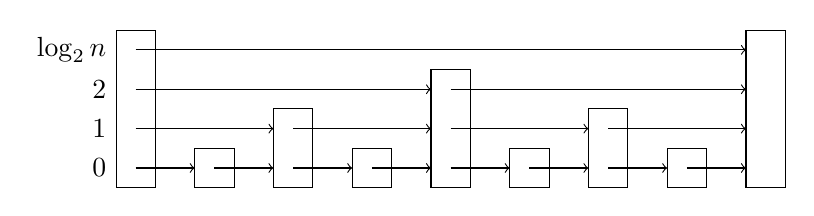
\begin{tikzpicture}[scale=.5]
    \draw
    (-2,0) rectangle (-1,4)

    (0,0) rectangle (1,1)
    (2,0) rectangle (3,2)
    (4,0) rectangle (5,1)
    (6,0) rectangle (7,3)
    (8,0) rectangle (9,1)

    (10,0) rectangle (11,2)
    (12,0) rectangle (13,1)

    (14,0) rectangle (15,4);

    \draw[->] (-1.5,.5) -- (0,.5);
    \draw[->] (0.5,.5) -- (2,.5);
    \draw[->] (2.5,.5) -- (4,.5);
    \draw[->] (4.5,.5) -- (6,.5);
    \draw[->] (6.5,.5) -- (8,.5);

    \draw[->] (8.5,.5) -- (10,.5);
    \draw[->] (10.5,.5) -- (12,.5);
    \draw[->] (12.5,.5) -- (14,.5);

    \draw[->] (-1.5,1.5) -- (2,1.5);
    \draw[->] (2.5,1.5) -- (6,1.5);
    \draw[->] (6.5,1.5) -- (10,1.5);
    \draw[->] (10.5,1.5) -- (14,1.5);

    \draw[->] (-1.5,2.5) -- (6,2.5);
    \draw[->] (6.5,2.5) -- (14,2.5);

    \draw[->] (-1.5,3.5) -- (14,3.5);

    \draw
    (-2,.5) node[left] {$0$}
    (-2,1.5) node[left] {$1$}
    (-2,2.5) node[left] {$2$}
    (-2,3.5) node[left] {$\floor{\log_2 n}$};
  \end{tikzpicture}
}

\begin{itemize}
  \item Zeiger auf Ebene $i$ zeigt zu nächstem $2^i$ Element
  \item Suchen $\in O(\log n)$
\end{itemize}

\begin{description}
  \item [Perfekt] Einfügen, Löschen $\in O(n)$
  \item [Randomisiert] Höhe zufällig \\ $P(h) = \frac{1}{2^{h + 1}}$: Einfügen, Löschen $\in O(\log n)$
\end{description}

\section{Sortierverfahren}

